\documentclass[notes,10pt, aspectratio=169]{beamer}

\usepackage{pgfpages}
% These slides also contain speaker notes. You can print just the slides,
% just the notes, or both, depending on the setting below. Comment out the want
% you want.
\setbeameroption{hide notes} % Only slide
%\setbeameroption{show only notes} % Only notes
%\setbeameroption{show notes on second screen=right} % Both
\usepackage{colortbl}
\usepackage{helvet}
\usepackage[default]{lato}
\usepackage{array}
\usepackage{eurosym}
\usepackage{setspace}
\usepackage{animate}
\usepackage{multicol}
\usepackage{breqn}
\usepackage{subcaption}
\usepackage{caption}
\captionsetup{font=scriptsize, justification=raggedright,singlelinecheck=false}
\usepackage[export]{adjustbox}
\usepackage[scale=2]{ccicons}
\usepackage{tikz}
\newenvironment{wideitemize}{\itemize\addtolength{\itemsep}{10pt}}{\enditemize}
\usepackage{natbib}
\usepackage{pgfplots}

\usepackage{tikz}
\usepackage{verbatim}
\setbeamertemplate{note page}{\pagecolor{yellow!5}\insertnote}
\usepackage{amsmath}
%\usepackage{mathpazo}
\usepackage{hyperref}
\usepackage{lipsum}
\usepackage{multimedia}
\usepackage{multirow}
\usepackage{graphicx}
\usepackage{dcolumn}
\usepackage{bbm}
\newcolumntype{d}[0]{D{.}{.}{5}}

\DeclareMathOperator{\CDF}{cdf}

\def\cdf(#1)(#2)(#3){0.5*(1+(erf((#1-#2)/(#3*sqrt(2)))))}%

\tikzset{
    declare function={
        normcdf(\x,\m,\s)=1/(1 + exp(-0.07056*((\x-\m)/\s)^3 - 1.5976*(\x-\m)/\s));
    }
}

\usepackage{changepage}
\usepackage{appendixnumberbeamer}
% \newcommand{\beginbackup}{
%   \newcounter{framenumbervorappendix}
%   \setcounter{framenumbervorappendix}{\value{framenumber}}
%   \setbeamertemplate{footline}
%   {
%      \leavevmode%
%      \hline
%      box{%
%       \begin{beamercolorbox}[wd=\paperwidth,ht=2.25ex,dp=1ex,right]{footlinecolor}%
% %         \insertframenumber  \hspace*{2ex} 
%       \end{beamercolorbox}}%
%      \vskip0pt%
%   }
%  }

 \setbeamertemplate{footline}{
    \hbox{%
    \begin{beamercolorbox}[wd=\paperwidth,ht=3ex,dp=1.5ex,leftskip=2ex,rightskip=2ex]{page footer}%
        %\usebeamerfont{title in head/foot}%
        %\insertshorttitle \hfill
        %\insertsection \hfill
        %\tableofcontents[currentsection] \hfill
        \insertsectionnavigationhorizontal{0.7\paperwidth}{}{} \hfill 
        \insertframenumber{} / \inserttotalframenumber
    \end{beamercolorbox}}%
}
\newcommand{\backupend}{
   \addtocounter{framenumbervorappendix}{-\value{framenumber}}
   \addtocounter{framenumber}{\value{framenumbervorappendix}} 
}

\useinnertheme[shadow]{rounded}
\setbeamercolor{block title example}{fg=black,bg=orange!50!white}
\setbeamercolor{block body example}{fg=black, bg=orange!30!white}
\setbeamercolor{block title alert}{fg=black,bg=green!50!white}
\setbeamercolor{block body alert}{fg=black, bg=green!30!white}
\setbeamercolor{block title}{use=structure,fg=structure.fg,bg=structure.fg!20!bg}
\setbeamercolor{block body}{parent=normal text,use=block title,bg=block title.bg!50!bg}

\newcommand\independent{\protect\mathpalette{\protect\independenT}{\perp}}
\def\independenT#1#2{\mathrel{\rlap{$#1#2$}\mkern2mu{#1#2}}}

\usepackage{graphicx}
\usepackage[space]{grffile}
\usepackage{booktabs}

% These are my colors -- there are many like them, but these ones are mine.
\definecolor{blue}{RGB}{0,114,178}
\definecolor{red}{RGB}{213,94,0}
\definecolor{yellow}{RGB}{240,228,66}
\definecolor{green}{RGB}{0,158,115}

\setbeamercolor{section in head/foot}{fg=blue}


\hypersetup{
  colorlinks=false,
  linkbordercolor = {white},
  linkcolor = {blue}
}


%% I use a beige off white for my background
\definecolor{MyBackground}{RGB}{255,253,218}

%% Uncomment this if you want to change the background color to something else
%\setbeamercolor{background canvas}{bg=MyBackground}

%% Change the bg color to adjust your transition slide background color!
\newenvironment{transitionframe}{
  \setbeamercolor{background canvas}{bg=yellow}
  \begin{frame}}{
    \end{frame}
}

\setbeamercolor{frametitle}{fg=blue}
\setbeamercolor{title}{fg=black}
%\setbeamertemplate{footline}[frame number]
\setbeamertemplate{navigation symbols}{} 
\setbeamertemplate{itemize items}{-}
\setbeamercolor{itemize item}{fg=blue}
\setbeamercolor{itemize subitem}{fg=blue}
\setbeamercolor{enumerate item}{fg=blue}
\setbeamercolor{enumerate subitem}{fg=blue}
\setbeamercolor{button}{bg=white,fg=blue,}



% If you like Traffic maps, rather than having clutter at the top, have a Trafficmap show up at the end of each section 
% (and after your introduction)
% Uncomment this is if you want the Trafficmap!
% \AtBeginSection[]
% {
%    \begin{frame}
%        \frametitle{Trafficmap of Talk}
%        \tableofcontents[currentsection]
%    \end{frame}
% }
\setbeamercolor{section in toc}{fg=blue}
\setbeamercolor{subsection in toc}{fg=red}
%\setbeamersize{text margin left=1em,text margin right=1em} 
\setbeamersize{text margin left=0.7cm,text margin right=0.7cm} 


\title[]{\textcolor{blue}{Lecture 11:\\An Introduction to Binary Choice Models}}
\author{25117 - Econometrics}
\institute[shortinst]{Universitat Pompeu Fabra}

\date{November 27nd, 2024}

\begin{document}

\begin{frame}[plain]
\maketitle
\end{frame}



\begin{frame}{What we learned in the last lesson}
\begin{itemize}
\item Panel data consist of observations on multiple ($n$) units -- states, firms, people, and so forth -- where each unit is observed at two or more time periods ($T$).
\item Regression with unit fixed effects controls for unobserved variables that differ from one entity to the next but remain constant over time.
\item Unit fixed effects regression can be estimated by including binary variables for $n - 1$ entities plus the observable independent variables (the $X$’s) and an intercept.
\item Time fixed effects control for unobserved variables that are the same across entities but vary over time.
\item A regression with time and entity fixed effects can be estimated by including binary variables for $n - 1$ entities and binary variables for $T - 1$ time periods plus the $X$’s and an intercept.
\item In panel data, variables are typically autocorrelated -- that is, correlated over time within an entity. Standard errors need to allow both for this autocorrelation and for potential heteroskedasticity, and one way to do so is to use clustered standard errors.
\end{itemize}
\end{frame}


\begin{frame}{Binary Choice Models}

So far the dependent variable $Y$ has been continuous:
\begin{itemize}
    \item district-wide average test score
    \item traffic fatality rate
\end{itemize}
\vspace{1em}
\begin{center}
    {\color{purple}\textbf{What if $Y$ is binary?}}
\end{center}
\begin{itemize}
    \item get into college, or not
    \item smoking, or not
    \item passing exams, or not
    \item mortgage application is accepted, or not
\end{itemize}
\vspace{1em}
\textbf{Example: Mortgage Denial and Race The Boston Fed HMDA Dataset}
\begin{itemize}
    \item $Y$ -- Is mortgage accepted?
    \item $X$ -- debt payments to income ratio (P/I ratio)
    \item other covariates -- race of applicant, wealth, employment status, other loan, property characteristics

\end{itemize}

\end{frame}


\begin{frame}{Binary Choice Models}
To study the relationship between a set of variables $x_i'$ and the dependent variable $y_i$, we need to extract information about:
\[
E[y_i \mid x_i']
\]
The conditional expectation in the familiar linear regression case is $E[y_i \mid x_i']=x_i'\beta$. \\~\\
In this topic, we will posit that the relationship between the vector of explanatory variables $x_i'$ and the dependent variable is not necessarily linear. In particular, we define:
\[
E[y_i \mid x_i']=F(x_i'\beta)
\]
So, a central element of this topic will be the choice of the distribution function $F$
\end{frame}

\begin{frame}{Linear Probability Model}
A natural starting point is the linear regression model with a single regressor:
\begin{equation*}
    Y_i = \beta_0 + \beta_1 X_i +u_i
\end{equation*}
In the linear probability model (LPM), the predicted value of $Y$ is interpreted as the predicted probability that $Y=1$ and $\beta_1$ is the change in that predicted probability for a unit change in $X$.\\[1em]

When $Y$ is binary,
\begin{equation*}
    \mathbb{E}(Y\mid X) = 1 \times Pr(Y=1\mid X) + 0 \times  Pr(Y=0\mid X) = Pr(Y=1\mid X)= \beta_0 + \beta_1 X_i
\end{equation*}\\[1em]

So $\hat{Y}$ is the predicted probability that $Y=1$ and $\beta_1$ is the difference in probability that $Y=1$ when $X$ increases by one unit.

\begin{equation*}
    \beta_1 = \frac{Pr(Y=1\mid X + \Delta X)-Pr(Y=1\mid X)}{\Delta X}
\end{equation*}\\[1em]
\end{frame}


\begin{frame}{Linear Probability Model}
Let's start by defining that $F(x_i'\beta)=x_i'\beta$. For example, if we have $k$ explanatory variables, the equation we aim to estimate will be:
\[
y_i=\beta_0+\beta_1x_{1,i}+\beta_2x_{2,i}+...+\beta_kx_{k,i}+u_i
\]
\begin{itemize}
    \item \textbf{Parameter Interpretation}: $\beta_j$ captures the change in $Pr(y_i=1)$ when $x_j$ increases by one unit.
    \[\frac{\partial y_i}{\partial x_{i,j}}=\beta_j\]
    \item \textbf{Estimation:} The parameter vector $\beta=\{\alpha, \beta_1,...,\beta_k\}$ is estimated using ordinary least squares (OLS).
    \[
    \beta^{OLS} = \underset{\beta}{arg \ max } \sum_{i=1}^n (y_i-x_i'\beta)^2 
    \]
\end{itemize}
\end{frame}

\begin{frame}{Properties of the Linear Probability Model}
\begin{itemize}
    \item \textbf{Conditional Expectation}: 
    \[
    E[y_i \mid x_i]=Pr[y_i=1 \mid x_i]=x_i'\beta
    \]  
    \item \textbf{Total Probability}: 
    \[
    Pr[y_i=0 \mid x_i]=1-x_i'\beta
    \]
    \item \textbf{Expectation of Errors:}
    \[
    Assumption: \ \ E[u_i \mid x_i']=0 
    \]
    \item \textbf{Error Variance (valid under the previous assumption)}: 
    \[
    Var(y_i \mid x_i)=x_i'\beta(1-x_i'\beta){\color{red} \ \ heteroscedasticity}
    \]
\end{itemize}
\end{frame}

\begin{frame}{Properties of the Linear Probability Model}
As we just mentioned, the error variance is heteroscedastic. In particular, we have:
\[
u_i=\begin{cases} 
      1-x_i'\beta & \text{if} \ \  y_i=1  \\
      -x_i'\beta & \text{if} \ \ y_i=0\\
\end{cases}
\]
And therefore:
\[
u_i=\begin{cases} 
      1-x_i'\beta & \text{with probability} \ \ x_i'\beta  \\
      -x_i'\beta & \text{with probability} \ \  1-x_i'\beta \\
\end{cases}
\]
\end{frame}

\begin{frame}{Linear Probability Model}
 \begin{columns}
\begin{column}{0.3\textwidth}
\begin{itemize}
    \item The linear probability model models $Pr(Y=1\mid X)$ as a linear function of $X$
    \item Is it a correct functional form?
    \item[$\rightarrow$] Here, mortgage denial v. ratio of debt payments to income (P/I ratio) in a subset of the HMDA data set (n = 127)
\end{itemize}
\end{column}
\begin{column}{0.75\textwidth}
\begin{figure}
  \centering
         \vspace{-1mm}
        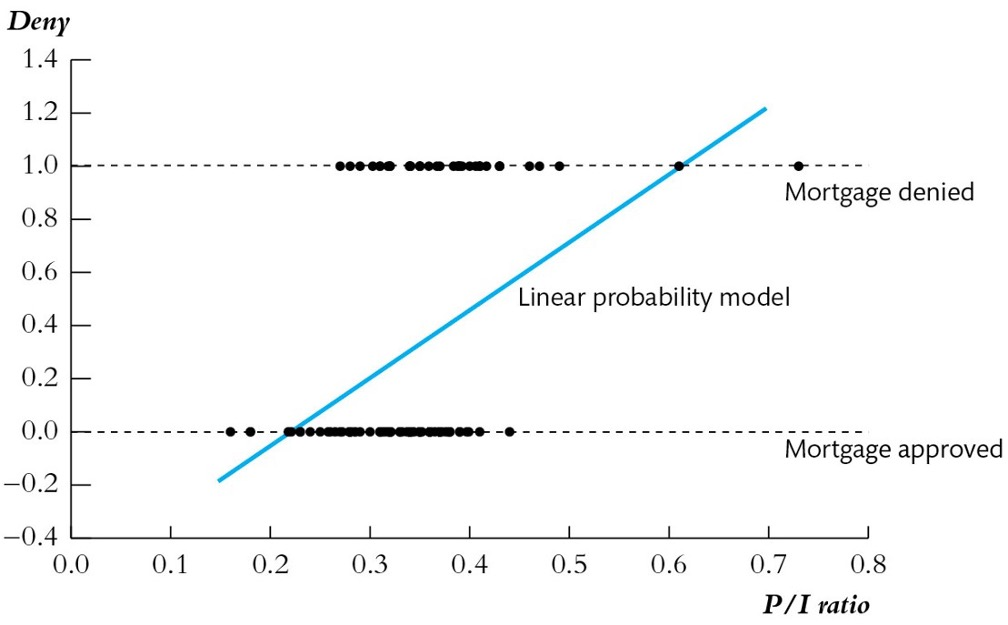
\includegraphics[scale=.3]{images/lpm.jpg}
\end{figure}
\end{column}
\end{columns}
\end{frame}

\begin{frame}{Linear Probability Model}

There advantages and disadvantages in modelling $Pr(Y=1\mid X)$ as a linear function of $X$
\begin{columns} 
% Column 1
    \begin{column}{.5\textwidth}
        \begin{center}
            \textbf{Pros}
        \end{center}
        \begin{itemize}
            \item Very simple to estimate and to interpret
            \item Statistical inference is the same as for multiple OLS regression (need heteroskedasticity-robust standard errors, etc.)
        \end{itemize}
    \end{column}
    \begin{column}{.5\textwidth}
        \begin{center}
            \textbf{Cons}
        \end{center}
        \begin{itemize}
        \setcounter{enumi}{7}
            \item A LPM says that the change in the predicted probability for a given change in $X$ is the same (percentage-point) for all values of $X$, but that does not make sense.
            \item LPM predicted probabilities can be larger than 1 and smaller than 0!

        \end{itemize}

    \end{column}
\end{columns}
\vspace{2em}

These disadvantages can be solved by using a nonlinear probability model...\\
\begin{center}
    $\longrightarrow$ probit and logit regressions
\end{center}
\end{frame}



\begin{frame}{Nonlinear Models}
 \begin{columns}
\begin{column}{0.4\textwidth}
The problem with the linear probability model is that it models the probability of $Y=1$ as a linear function of $X$:
\begin{equation*}
     Pr(Y=1\mid X)= \beta_0 + \beta_1 X_i
\end{equation*}
Instead, we want:
\begin{itemize}
    \item $Pr(Y=1\mid X)$ increases with $X$ if $\beta_1$ is positive
    \item $0\leq Pr(Y=1\mid X)\leq1 \forall X$ 
\end{itemize}
\end{column}
\begin{column}{0.6\textwidth}
\begin{figure}
  \centering
         \vspace{-1mm}
        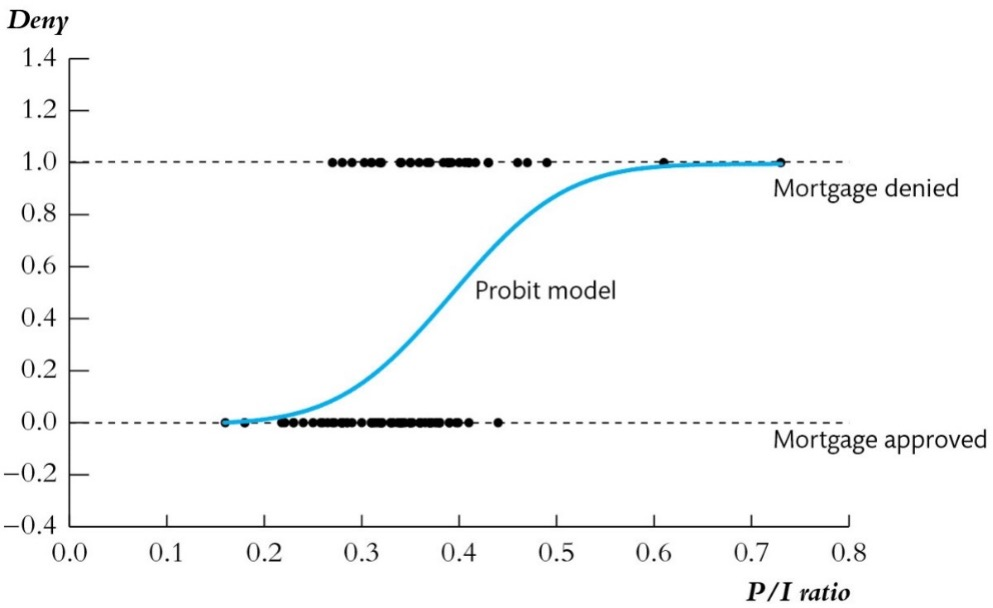
\includegraphics[scale=.25]{images/probit0.jpg}
\end{figure}
\end{column}
\end{columns}
This requires using a nonlinear functional form for the probability... Probit and Logit models satisfies these conditions
\end{frame}


\begin{frame}{Nonlinear Models}
So far, we have treated $Pr(y_i=1 \mid x_i')$ linearly. Now, assume that this probability is given by a distribution function $F(x_i'\beta)$. \\[1em]
To introduce the distribution of the variable $y_i$, consider the following latent variable model:
\[
y_i^*=x_i'\beta+\varepsilon_i
\]
If in this latent variable model $y_i^*$ is positive, then $y_i=1$, and if $y_i^*$ is negative, then $y_i=0$. In this case:
\[
Pr(y_i=1 \mid x_i)=Pr(y_i^*>0 \mid x_i)=Pr(\varepsilon_i>-x_i'\beta\mid x_i)=F(x_i'\beta)
\]
Therefore, when choosing the distribution function of errors in the latent model, we are determining how the probability of choosing an alternative behaves.
\end{frame}


\begin{frame}{Probit Model}
Probit regression models the probability that $Y=1$ using the cumulative standard  \textit{normal} distribution function, $\Phi(z)$, evaluated at $z=\beta_0 + \beta_1 X_1$. So the probit regression model reads:
\begin{equation*}
     Pr(Y=1\mid X_i)= \Phi(\beta_0 + \beta_1 X_i) = \frac{1}{\sqrt{2\pi}}\int^{\beta_0 + \beta_1 X_i}_{-\infty} e^{-t^2/2}dt
\end{equation*}

\textbf{Example:} Suppose that $\beta_0 = -3.5$ and $\beta_1 = 2$. Then

\begin{equation*}
     Pr(Y=1\mid X=.61)= \Phi(-3.5 + 2 \times .61)=\Phi(-2.28)=0.0113
\end{equation*}
$Pr(Y=1\mid X=.61)$ corresponds to the area under the standard normal density to left of $z=-2.28$
\end{frame}


\begin{frame}{Probit Model}
\begin{figure}
  \centering
         \vspace{-1mm}
        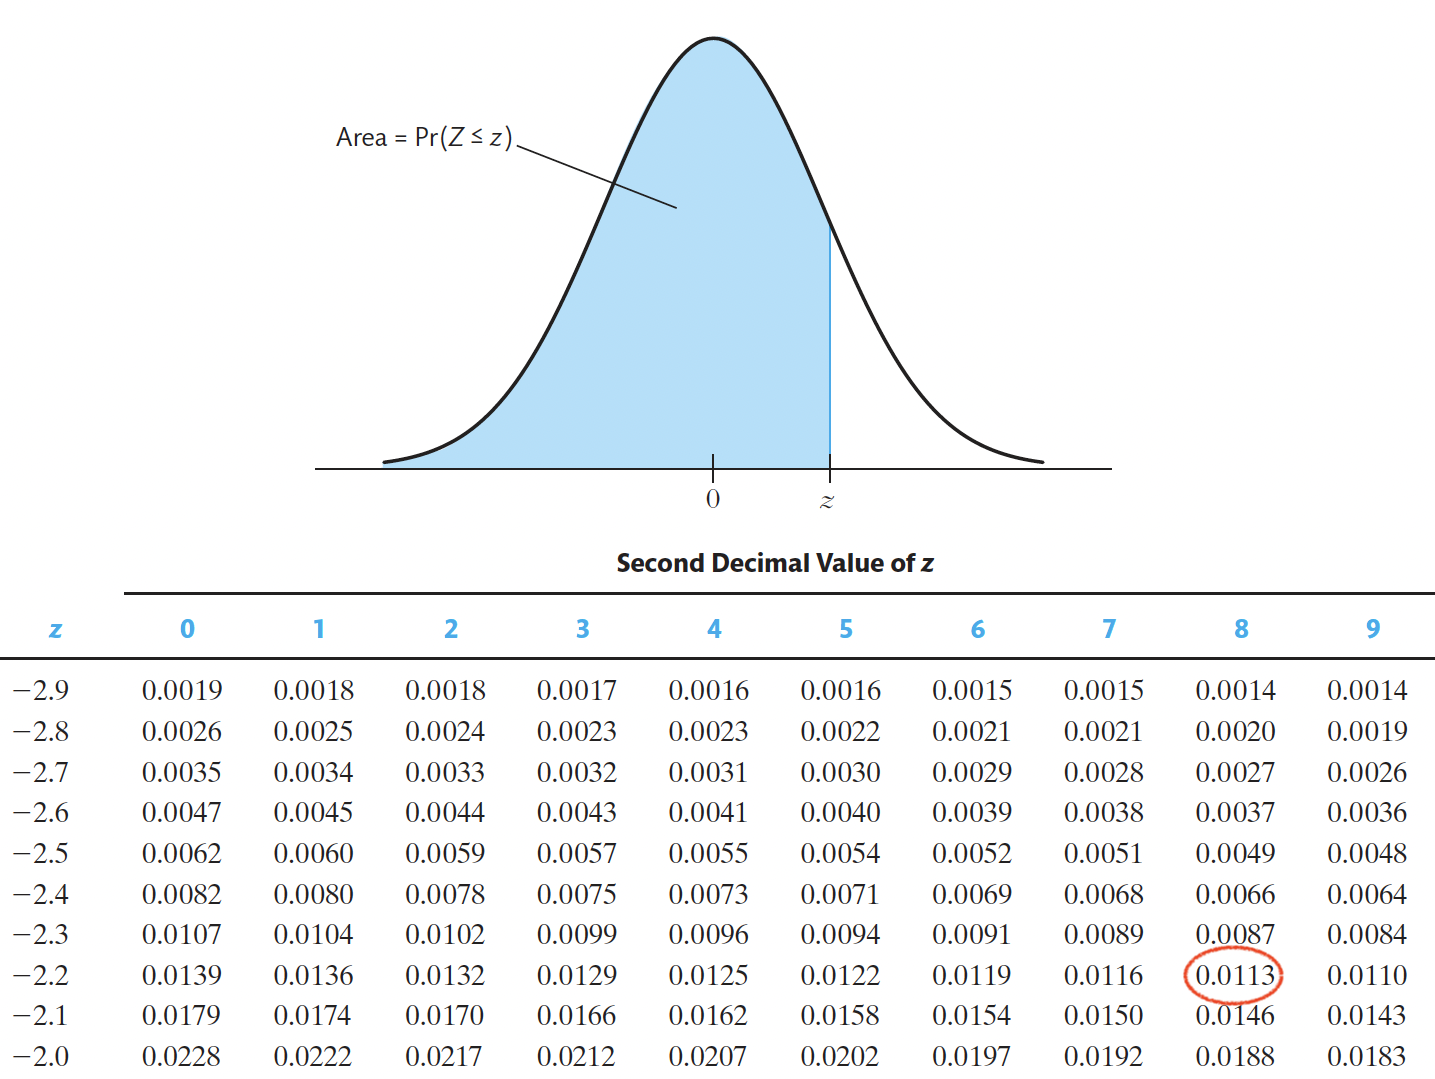
\includegraphics[scale=.4]{images/normal_pdf.png}
\end{figure}
\end{frame}

\begin{frame}{Logit Model}
Logit regression models the probability that $Y=1$ using the cumulative standard \textit{logistic} distribution function, $F(z)$, evaluated at $z=\beta_0 + \beta_1 X_1$. So the logit regression model reads:
\begin{equation*}
     Pr(Y=1\mid X_i)= F(\beta_0 + \beta_1 X_i) =\frac{e^{\beta_0 + \beta_1 X_i}}{1+e^{\beta_0 + \beta_1 X_i}}=\frac{1}{1+e^{-(\beta_0 + \beta_1 X_i)}}
\end{equation*}

\textbf{Example:} Suppose (again) that $\beta_0 = -3.5$ and $\beta_1 = 2$. Then

\begin{equation*}
     Pr(Y=1\mid X=.61)= F(-3.5 + 2 \times .61)=\frac{1}{1+e^{2.28}}=0.0928
\end{equation*}
$Pr(Y=1\mid X=.61)$ corresponds to the area under the standard \textit{logistic} density to left of $z=-2.28$\\[1em]

Because logit and probit use different probability functions, the coefficients $\beta$s are different and have different interpretations...
\end{frame}

\begin{comment}
\begin{frame}{Coefficients interpretation -- Probit}
\begin{figure}
  \centering
         \vspace{-1mm}
        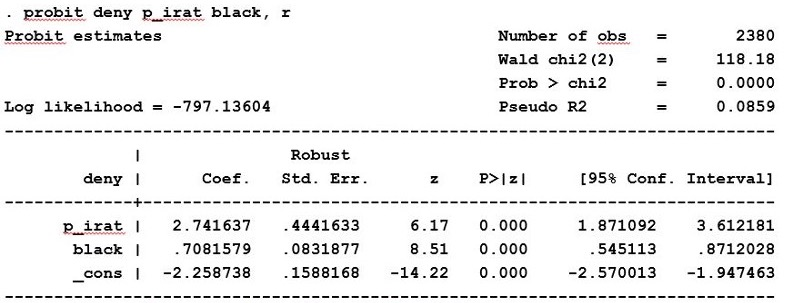
\includegraphics[scale=.5]{images/probit2.jpg}
\end{figure}
How can we interpret these coefficients?
\end{frame}


\begin{frame}{Coefficients interpretation -- Probit}
Interpreting coefficients from a probit model is not straightforward. Here, imagine the case of a white person with a P/I ratio of .3. Then,
\begin{eqnarray*}
    &Pr(\text{denied}=1\mid \text{P/I ratio}=0.3, \text{black}=0)&= \Phi(-2.259 + 0.3 \times 2.741 + 0 \times 0.708)\\
    &{} &=\Phi(-1.436)=0.075
\end{eqnarray*}  
A 50 percentage-point increase in the P/I ratio, \textit{ceteris paribus}, would yield:
\begin{eqnarray*}
    &Pr(\text{denied}=1\mid \text{P/I ratio}=0.8, \text{black}=0)&= \Phi(-2.259 + 0.8 \times 2.741 + 0 \times 0.708)\\
    &{} &=\Phi(-0.065)=0.474
\end{eqnarray*}  
So, conditional on being a white person, an increase in the P/I ratio from 0.3 to 0.8 is associated with an increase in the probability of mortgage denial from .075 to .474.\\[1em]

But conditional on being a white person, an increase in the P/I ratio from 0 to 0.5 is associated with an increase in the probability of mortgage denial from .012 to .187 (non-linear marginal effects!)
\end{frame}


\begin{frame}{Coefficients interpretation -- Probit}
Let's study the same case, now for a black person. Then,
\begin{eqnarray*}
    &Pr(\text{denied}=1\mid \text{P/I ratio}=0.3, \text{black}=1)&= \Phi(-2.259 + 0.3 \times 2.741 + 1 \times 0.708)\\
    &{} &=\Phi(-0.728)=0.233
\end{eqnarray*}  
A 50 percentage-point increase in the P/I ratio, \textit{ceteris paribus}, would yield:
\begin{eqnarray*}
    &Pr(\text{denied}=1\mid \text{P/I ratio}=0.8, \text{black}=1)&= \Phi(-2.259 + 0.8 \times 2.741 + 1 \times 0.708)\\
    &{} &=\Phi(0.643)=0.74
\end{eqnarray*}  
So, conditional on being a black person, an increase in the P/I ratio from 0.3 to 0.8 is associated with an increase in the probability of mortgage denial from .233 to .74.\\[1em]

But conditional on being a white person, an increase in the P/I ratio from 0 to 0.5 is associated with an increase in the probability of mortgage denial from .06 to .43 (again, non-linear marginal effects!)
\end{frame}

\begin{frame}{Coefficients interpretation -- Logit}
\begin{figure}
  \centering
         \vspace{-1mm}
        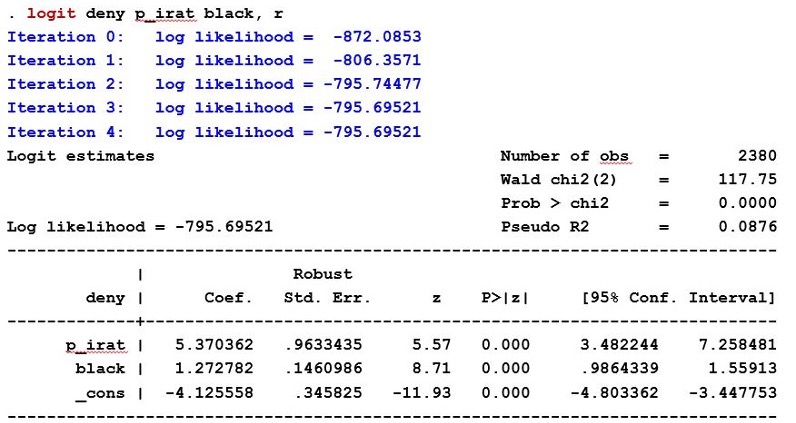
\includegraphics[scale=.5]{images/logit2.jpg}
\end{figure}
%How can we interpret these coefficients?
\end{frame}


\begin{frame}{Coefficients interpretation -- Logit}
Interpreting coefficients from a logit model is way simpler. Again, imagine the case of a white person with a P/I ratio of .3. Then,
\begin{eqnarray*}
    &Pr(\text{denied}=1\mid \text{P/I ratio}=0.3, \text{black}=0)&= F(-4.126 + 0.3 \times 5.37 + 0 \times 1.273)\\
    &{} &=F(-2.514)=0.075
\end{eqnarray*}  
It is the (almost) the same as before! A 50 percentage-point increase in the P/I ratio, \textit{ceteris paribus}, would yield:
\begin{eqnarray*}
    &Pr(\text{denied}=1\mid \text{P/I ratio}=0.8, \text{black}=0)&= F(-4.126 + 0.3 \times 5.37 + 0 \times 1.273)\\
    &{} &=F(.17)=.543
\end{eqnarray*}  
So, conditional on being a white person, an increase in the P/I ratio from 0.3 to 0.8 is associated with an increase in the probability of mortgage denial from .075 to .543.\\[1em]

Again, conditional on being a white person, an increase in the P/I ratio from 0 to 0.5 is associated with an increase in the probability of mortgage denial from .016 to .808.
\end{frame}

\end{comment}

\begin{frame}{Marginal Effects}
The \textit{probit} and \textit{logit} estimates provide the vector $\beta$, but not the marginal effects, which are:

 \[
    \frac{\partial \Phi(x_i'\beta)}{\partial x_k}=\beta_k\phi(x_i'\beta) \ \ \ Probit
    \]
\[
    \frac{\partial \frac{e^{x_i'\beta}}{1+e^{x_i'\beta}} }{\partial x_k}=\beta_kPr(y_i=1)(1-Pr(y_i=1)) \ \ \ Logit
    \]
Therefore, to evaluate the marginal effects, we need to provide values to $x_i'$. In Stata, we calculate the marginal effects using the \texttt{margins} function after estimating the corresponding model. With this function, Stata calculates the average marginal effects, i.e.:
\[
\frac{1}{n}\sum_i \frac{\partial E[y_i \mid x_i]}{\partial x_k}
\]
\end{frame}


\begin{frame}{Marginal Effects}
A distinction must be made between:\\~\\
\begin{enumerate}
    \item Average marginal effects: obtain the marginal effect on each individual and then calculate the average of the marginal effects
    \[
\frac{1}{n}\sum_i \frac{\partial E[y_i \mid x_i]}{\partial x_k}
\]
\item Marginal effects calculated at the mean: obtain the marginal effect by evaluating the expression at the mean of the explanatory variables:
\[
\frac{\partial E[y_i \mid x_i]}{\partial x_k} \mid_{x_i=\bar{x}}
\]
Since $E[y_i \mid x_i]$ is not linear in $x_i$, the two calculations yield different results. 
\end{enumerate}

\end{frame}


\begin{frame}{Marginal Effects (Logit)}
    \begin{figure}[H]
    \centering
    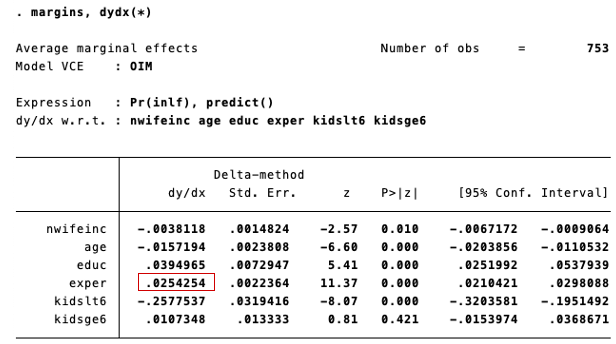
\includegraphics[scale=0.45]{images/LogitMargins.png}
    \label{fig:my_label}
\end{figure}
\end{frame}

\begin{frame}{Marginal Effects (Logit)}
    \begin{figure}[H]
    \centering
    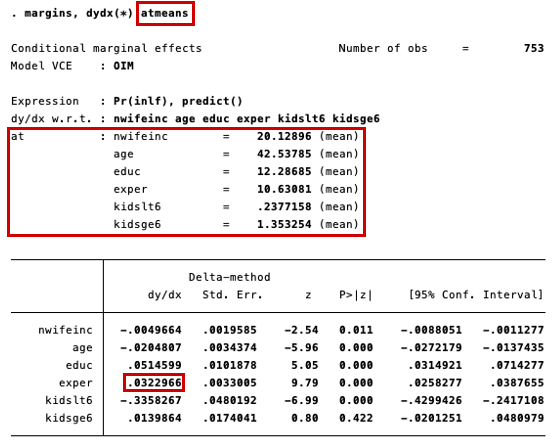
\includegraphics[scale=0.45]{images/AtmeansLogit.png}
    \label{fig:my_label}
\end{figure}
\end{frame}


\begin{frame}{So... Probit or Logit?}
\begin{figure}
  \centering
         \vspace{-1mm}
        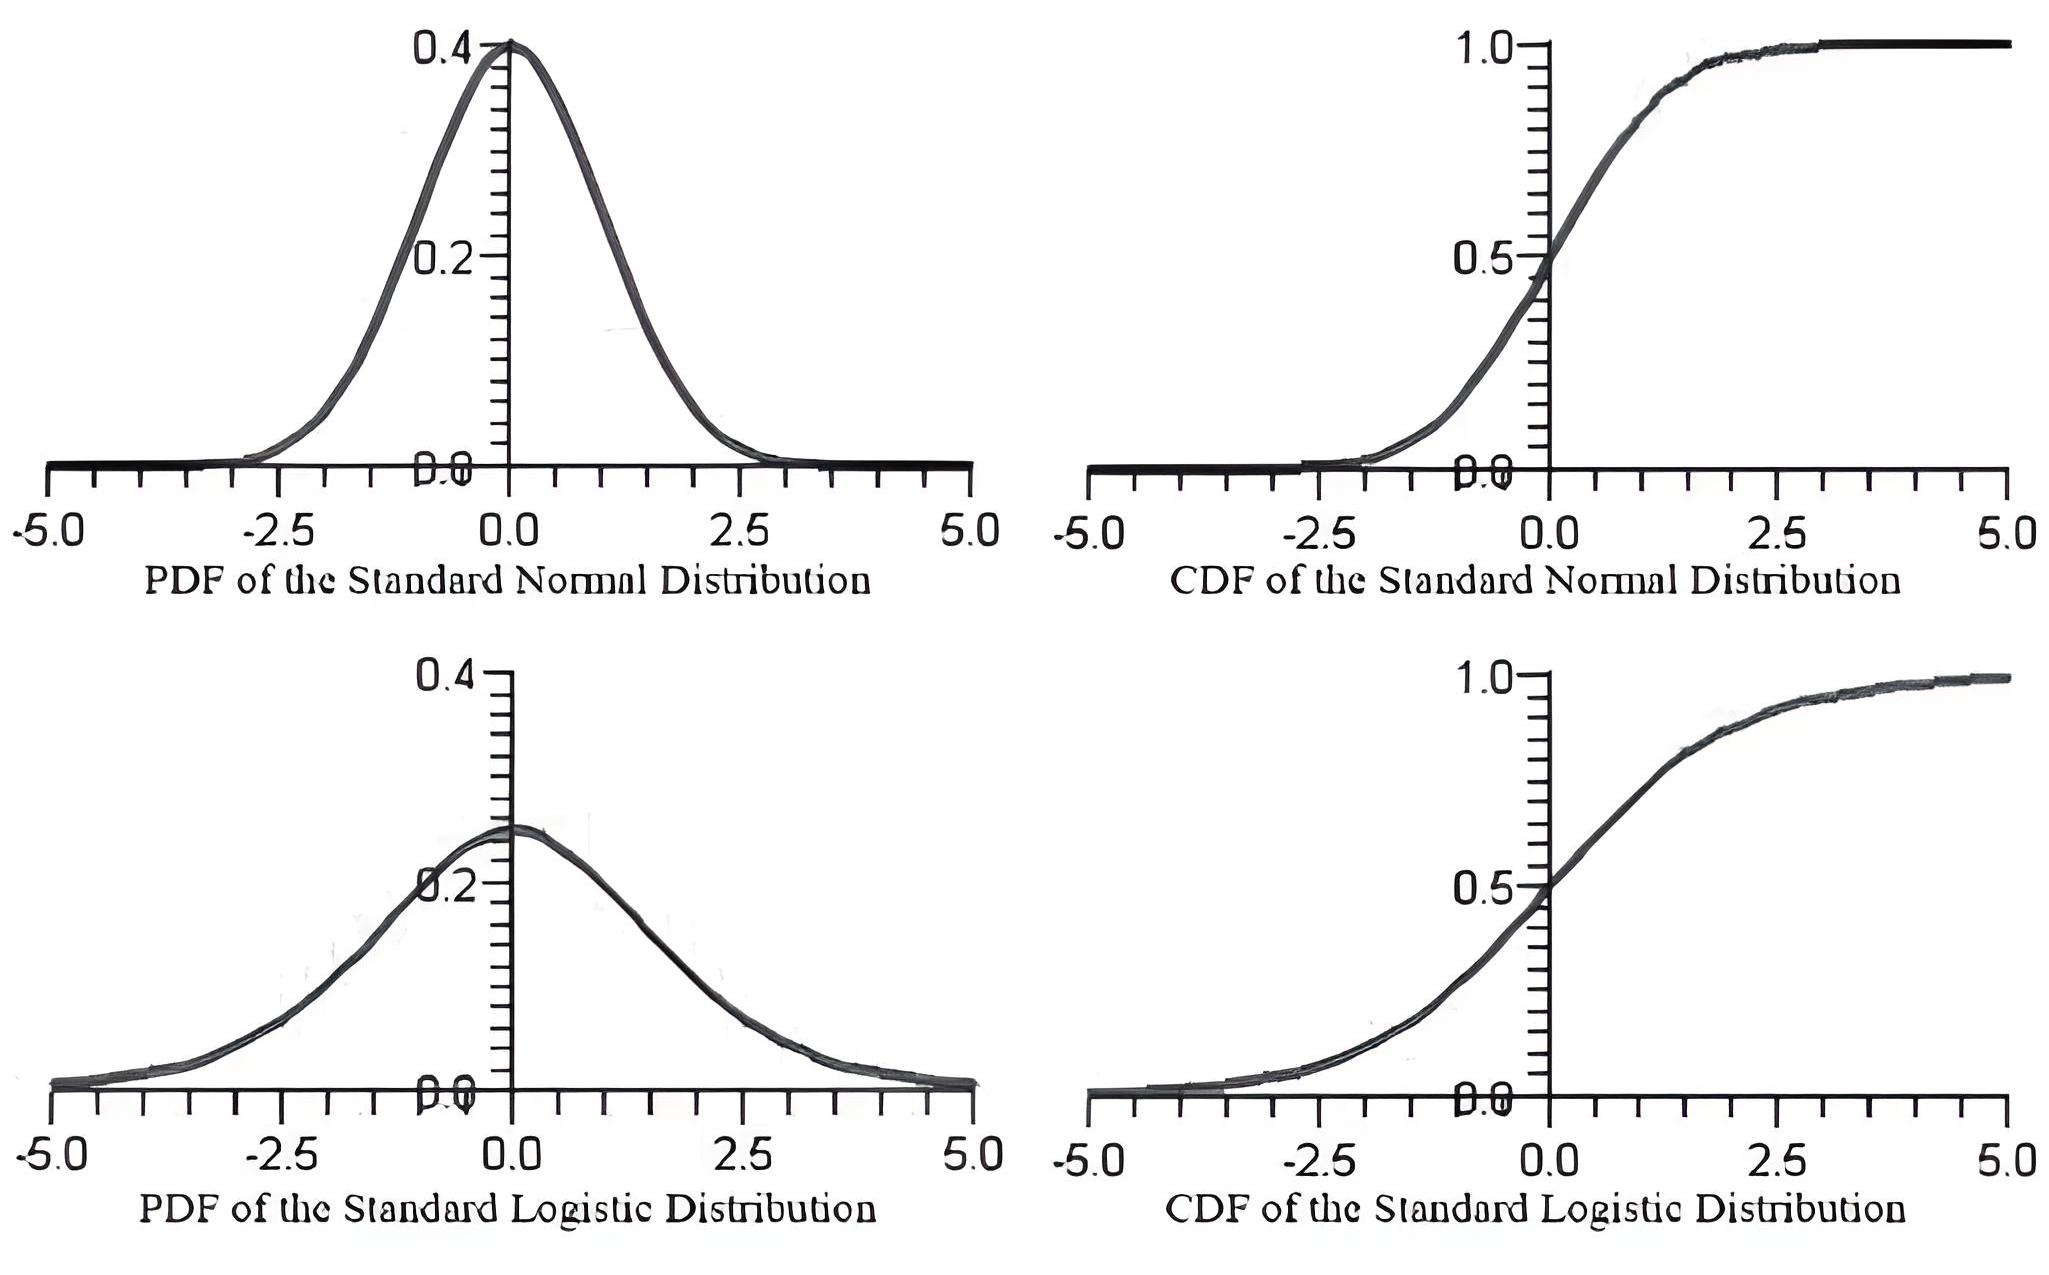
\includegraphics[scale=.15]{images/logisticnormal.jpeg}
\end{figure}
\end{frame}

\begin{frame}{Solution to Fitted Probabilities}
\begin{figure}[H]
    \centering
    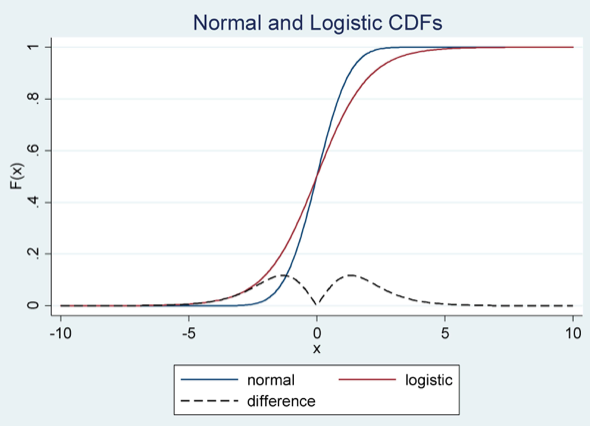
\includegraphics[scale=0.45]{images/Cdf's.png}
    \label{fig:my_label}
\end{figure}  
\end{frame}


\begin{frame}{So... Probit or Logit?}
Why do we have two different models? The main reason is historical: logit is computationally faster and easier, but that doesn't matter nowadays with modern computation softwares.\\[1em]

Now, the logistic distribution displays fatter tails (i.e the probit curve approaches the axes more quickly than the logit curve.)\\[1em]

This matters for extremes, but in practice, logit and probit are very similar when the binary outcome is decently balanced (perfectly balanced 50\% 0s, 50\% 1s)\\[1em]

This is the case in the vast majority of the applications...\\[1em]

Logit models tend to be slightly more used in practice because the $\beta$s are easier to interpret: they are in log-odds units ($ln(\frac{Pr(Y=1|X)}{1-Pr(Y=1|X)})$).\\[1em]

\end{frame}


\begin{frame}{Log-Odds-Ratio}
Suppose that:
\[
\frac{Pr(y_i=1)}{Pr(y_i=0)}=1.1 \implies \textit{The probability of choosing 1 is 10\% greater than choosing 0}
\]\\~\\
In terms of log-odds ratio (assuming odds ratio is close to 1):\\
\[
ln(Pr(y_i=1))-ln(Pr(y_i=0))\approx 0.1
\]\\
Also indicates that the probability of choosing $1$ over $0$ is 10\% greater.\\~\\
\begin{itemize}
    \item Important: if $\beta_k>0$:
    \[
    \frac{\partial odds}{\partial x_k}>0 \ \ \&  \ \ \frac{\partial log-odds }{\partial x_k}>0
    \]
\end{itemize}
\end{frame}


\begin{frame}{Why log-odds units?}
\begin{eqnarray*}
    &Pr(Y=1\mid X_i)&= F(\beta_0 + \beta_1 X_i) =\frac{e^{\beta_0 + \beta_1 X_i}}{1+e^{\beta_0 + \beta_1 X_i}}\\
& \Leftrightarrow & \frac{1}{Pr(Y=1\mid X_i)} = \frac{1+e^{\beta_0 + \beta_1 X_i}}{e^{\beta_0 + \beta_1 X_i}}=1+\frac{1}{e^{\beta_0 + \beta_1 X_i}}\\
& \Leftrightarrow & \frac{1 - Pr(Y=1\mid X_i)}{Pr(Y=1\mid X_i)}  =\frac{1}{e^{\beta_0 + \beta_1 X_i}}\\
& \Leftrightarrow & \frac{Pr(Y=1\mid X_i)}{1 - Pr(Y=1\mid X_i)}  =e^{\beta_0 + \beta_1 X_i}\\
& \Leftrightarrow & ln\Bigg[\frac{Pr(Y=1\mid X_i)}{1 - Pr(Y=1\mid X_i)}\Bigg]  =\beta_0 + \beta_1 X_i\\
\end{eqnarray*}
Using the preceding example, a 10\%-point increase in the P/I ratio, \textit{ceteris paribus}, would yield a 0.537 ($.1\times5.37$) increase in the log odds of being denied a mortgage... Put differently, the odds (p/(1-p)) of being denied a mortgage would increase by 71\% ($e^{0.537}=1.71$) !
\end{frame}


%MLE
%Goodness of fit
% Other models (truncated, poisson, etc.
\section{Maximum Likelihood Estimation}

\begin{frame}
  \vfill
  \centering
    {\huge \color{blue} \textit{Maximum Likelihood Estimation}}
  \vfill
\end{frame}

\begin{frame}{Estimation and Inference in the Logit and Probit Models}
In your previous lectures, you were assuming regression models that are linear or nonlinear (e.g., polynomials) functions of the independent variables but are linear functions of the unknown coefficients (parameters) $\rightarrow$ can be estimated by OLS.\\[1em]
In contrast, the probit and logit regression functions are nonlinear
functions of the coefficients $\rightarrow$ cannot be estimated by OLS $\rightarrow$ {\color{green} NEW METHOD:} \textbf{Maximum Likelihood}\\[1em]
Maximum Likelihood Estimation (MLE) in econometrics is a method for estimating the parameters of a statistical model by maximizing the likelihood function.\\[1em]
The likelihood function represents the probability of observing the given sample data under different parameter values.\\[1em]
Formally, MLE seeks to find the parameter values that maximize the likelihood function, or equivalently, minimize the negative log-likelihood.\\[1em]
\end{frame}




\begin{frame}{Estimation and Inference in the Logit and Probit Models}
This process is akin to searching for the parameter values that make the observed data most probable, treating the sample as a realization of a probability distribution determined by the model.\\[1em]
The theory of ML says that the ML estimator $\hat{p}^{MLE}$ is the most efficient estimator of $p$ --- of \textit{all} consistent estimators! --- at least for large $n$. (Much stronger than the Gauss-Markov theorem!).\\[1em]
For this reason, the MLE is the primary estimator used for models in which the parameters (coefficients) enter nonlinearly. \\[1em]
In large samples, the MLE is:
\begin{itemize}
    \item Consistent
    \item Normally distributed
    \item Efficient (has the smallest variance of all consistent estimators)
\end{itemize}



\end{frame}



\begin{frame}{Bernoulli example}
  \begin{itemize}
    \item Suppose that we know that the following ten numbers were simulated using a Bernoulli distribution: $0, 0, 0, 1, 1, 0, 0, 1, 0, 1$.\\[1em]
    \item Denote them by $y_1, y_2, \ldots, y_{10}$. So $y_1=0$ and $y_{10}=1$\\[1em]
    \item The probability of 1 is $p$, while the probability of 0 is $(1 - p)$.\\[1em]
    \item Recall that the pdf of a Bernoulli random variable is $f(y; p) = p^y (1 - p)^{1-y}$, where $y \in \{0, 1\}$\\[1em]
    \item We want to find the $p$ that was used to simulate the ten numbers.\\[1em]
    \item \textbf{All we know} is that 1) they are drawn from a Bernoulli distribution and 2) independently from each other
  \end{itemize}
\end{frame}

\begin{frame}{Bernoulli example (contd.)}
  \begin{itemize}
    \item Since we know the pdf that generated the numbers is Bernoulli, we know that the probability of the \textit{first} number is $f(y_1; p) = p^{y_1} (1 - p)^{1-{y_1}}$\\[1em]
    \item ... and we know that the probability of the \textit{second}  number is $f(y_2; p) = p^{y_2} (1 - p)^{1-{y_2}}$, etc.\\[1em]
    \item We could replace the $y_i$ with the actual numbers. For example, the first one is $y_1 = 0$, so the probability is just $(1-p)$.\\[1em]
    \item What we do not know is \textbf{the value of the parameter} $p$\\[1em]
    \item Since we know that they are independent, we could also write down the probability of observing \underline{all ten numbers}. That is, their \textbf{joint probability}.\\[1em]
    \item Since they are independent, their joint probability distribution is the multiplication of the ten pdfs: $P(A\cap B) = P(A) \times P(B)$
  \end{itemize}
\end{frame}


\begin{frame}{Bernoulli example (contd.)}
  \begin{itemize}
    \item Since they are independent, we could write down the joint probability or the \textbf{likelihood} ($L$) of seeing those 10 numbers as:
    \[ L(p) = \prod_{i=1}^{10} p^{y_i} (1 - p)^{1 - y_i} \]
    \item We want to find the $\hat{p}$ that maximizes the likelihood function $L(p)$, i.e., the probability of observing all ten $y_i$\\[1em]
    \item Taking that derivative is complicated because we would need to use the chain rule several times so we take the log to simplify the notation. The log function is a \underline{monotonic} transformation, it won’t change the optimal $\hat{p}$:
    \[ \ln L(p) = \sum_{i=1}^{n} y_i \ln(p) + \sum_{i=1}^{n} (1 - y_i) \ln(1 - p) \]
  \end{itemize}
\end{frame}

\begin{frame}{Bernoulli example (contd.)}
  \begin{itemize}
    \item In this case, the log-likelihood function simplifies to
    \[ \ln L(p) = n \Bar{y} \ln(p) + n (1 - \Bar{y}) \ln(1 - p) \]\\[1em]
    \item Taking the derivative with respect to $p$ and setting it to zero, we find the MLE estimator of $p$:
    \[ \frac{\partial \ln(p)}{\partial p} = \frac{\bar{y}}{p} - \frac{1 - \bar{y}}{1 - p} = 0 \]\\[1em]
    \item Solving, we find that $\hat{p} = \bar{y} = \sum_{i=1}^{n} y_i / n$.\\[1em]
    \item So that’s the MLE estimator of p. This is saying more or less the obvious: our best guess for the p that generated the data is the proportion of 1s; in this case $p = 0.4$
  \end{itemize}
\end{frame}

% \begin{frame}{Maximum Likelihood Estimation (MLE)}
% Maximize the log likelihood by setting the derivative to zero $\frac{\partial ln[f(p)]}{\partial p} = 0$.\\[1em]

% In this case, 
% \begin{eqnarray*}
%     &\frac{\partial ln[f(p)]}{\partial p} &= \sum_{i=1}^n y_i \frac{1}{\hat{p}^{MLE}}-(n-\sum_{i=1}^n y_i)\frac{1}{1-\hat{p}^{MLE}}=0\\
%     &\Leftrightarrow & \frac{\sum_{i=1}^n y_i}{n-\sum_{i=1}^n y_i} = \frac{\hat{p}^{MLE}}{1-\hat{p}^{MLE}}\\
%     &\Leftrightarrow & \frac{\Bar{Y}}{1-\Bar{Y}} = \frac{\hat{p}^{MLE}}{1-\hat{p}^{MLE}}\Leftrightarrow \hat{p}^{MLE}=\Bar{Y}
% \end{eqnarray*}

% So, for $Y_i$ i.i.d Bernouilli, $\Bar{Y}$ is the MLE, the ``natural'' estimator of $p$\\[1em]

% In large $n$, the sampling distribution of  $\hat{p}^{MLE}$ is normally distributed. Thus, inference is “as usual”: hypothesis testing via t-test statistic, confidence interval as $1.96\times SE$, etc.
% \end{frame}


\begin{frame}{Maximum Likelihood Estimation (MLE)}
Analogously, the probit likelihood function is the joint density of $Y_1, Y_2, \dots, Y_n$ given $X_1=x_1, X_2=x_2, \dots, X_n=x_n$ treated as function of the unknown parameters $\beta_0, \beta_1$ (for only one regressor):
\begin{eqnarray*}
    &f(\beta_0, \beta_1; Y_1, Y_2, \dots, Y_n \mid X_1, X_2, \dots, X_n) &= \{[\Phi(\beta_0 + \beta_1 x_1)]^{y_1}\times[1-\Phi(\beta_0 + \beta_1 x_1)]^{1-y_1}\}\\
    &{} &\times\{[\Phi(\beta_0 + \beta_1 x_2)]^{y_2}\times[1-\Phi(\beta_0 + \beta_1 x_2)]^{1-y_2}\}\\
    &{} &\times\dots\\
    &{} &\times\{[\Phi(\beta_0 + \beta_1 x_n)]^{y_n} \times[1-\Phi(\beta_0 + \beta_1 x_n)]^{1-y_n}\}
\end{eqnarray*}
The parameters $\hat{\beta}^{MLE}_0, \hat{\beta}^{MLE}_1$ maximize this likelihood function!\\[1em]

We can easily extend this to multiple regressors and/or the logistic regression model...
\end{frame}


\begin{frame}{Maximum Likelihood Estimation (MLE)}
The logit likelihood function is the joint density of $Y_1, Y_2, \dots, Y_n$ given $X_1=x_1, X_2=x_2, \dots, X_n=x_n$ treated as function of the unknown parameters $\beta_0, \beta_1$ (for only one regressor):
\begin{eqnarray*}
    &f(\beta_0, \beta_1; Y_1, Y_2, \dots, Y_n \mid X_1, X_2, \dots, X_n) &= \{[F(\beta_0 + \beta_1 x_1)]^{y_1}\times[1-F(\beta_0 + \beta_1 x_1)]^{1-y_1}\}\\
    &{} &\times\{[F(\beta_0 + \beta_1 x_2)]^{y_2}\times[1-F(\beta_0 + \beta_1 x_2)]^{1-y_2}\}\\
    &{} &\times\dots\\
    &{} &\times\{[F(\beta_0 + \beta_1 x_n)]^{y_n} \times[1-F(\beta_0 + \beta_1 x_n)]^{1-y_n}\}
\end{eqnarray*}
In both cases, we cannot solve for the maximum explicitly! So, the MLE must be maximized using numerical methods (dynamic optimization algorithms).
\end{frame}


\begin{frame}{Model Selection Criteria}
When comparing two models that contain the same set of variables, we only need to examine the values of the likelihood functions. The higher, the better the model fits.\\~\\
There are different methods for choosing between models that do not have the same explanatory variables:
\begin{enumerate}
    \item Likelihood Ratio Test
    \item Number of correct predictions
    \item McFadden's $R^2$
    \item Akaike Information Criterion (AIC)
    \item Weighted Residual Sum of Squares
\end{enumerate}
\end{frame}

\begin{frame}{Model Selection Criteria}
\begin{itemize}
    \item Likelihood Ratio Test:
    \[
    LR=2[\mathcal{L}(\hat{\beta}_N)-\mathcal{L}(\hat{\beta}_R)] \sim \chi_q^2
    \]
Where N and R represent the unrestricted and restricted (i.e., without explanatory variables) models respectively, and q is the difference in parameters. If we reject $H_0$, the unrestricted model will be better. \\[1em]

\item Number of correct predictions: we assign $\hat{y}_i=1$ if $\hat{P}_i>a$ and count the number of incorrect predictions from the model $\sum_{i=1}^N (y_i-\hat{y}_i)^2$\\[1em]
\item $WSSR=\sum_{i=1}^n \frac{(y_i-\hat{P}_i)^2}{\hat{P}_i(1-\hat{P}_i)}$. The model that minimizes this is preferable.
\end{itemize}
\end{frame}

\begin{frame}{Model Selection Criteria}
\begin{itemize}
    \item Akaike Information Criterion (AIC): $AIC=-ln(\mathcal{L})+K$, where K is the number of estimated parameters. The smaller the AIC, the better.\\~\\
    \item McFadden's $R^2$: $R^2=1-\frac{ln(\mathcal{L}_N)}{ln(\mathcal{L}_R)} \in [0,1]$, where $L_R$ is the value of the likelihood function when only a constant is included, and $L_N$ is that of the unrestricted model.
\end{itemize}
\end{frame}



\begin{frame}{Application: Women's Participation in the Labor Market}
Dependent Variable $y_i\to \textit{inlf} \in \{0,1\}$ (0 if the woman is not in the labor market, 1 if she is)

\vspace{1em}
Explanatory Variables $x_i': (nwifeinc,educ,exp,exp^2,age,kidslt6,kidsge6)$

\vspace{1em}
\begin{itemize}
\item LPM:
\[
E[infl_i \mid x_i]=x_i'\beta
\]
\item  Probit:
\[
E[infl_i \mid x_i]=\Phi(x_i'\beta)
\]
\item Logit:
\[
E[infl_i \mid x_i]=\frac{e^{x_i'\beta}}{1+e^{x_i'\beta}}
\]
\end{itemize}
\end{frame}

\begin{frame}{LPM}
    \begin{figure}[H]
    \centering
    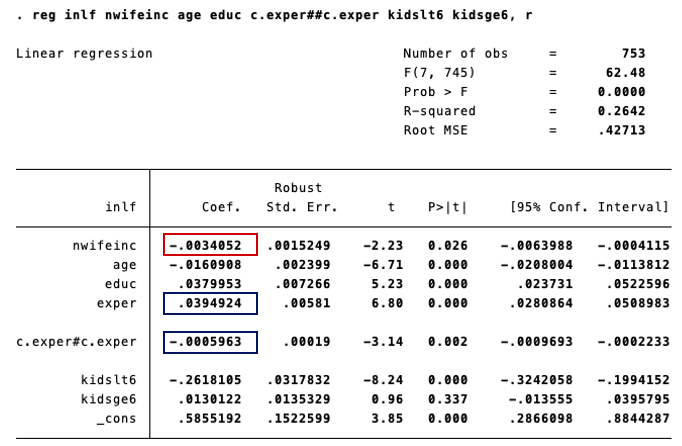
\includegraphics[scale=0.4]{images/LPMStata.png}
    \label{fig:my_label}
\end{figure}    
\end{frame}

\begin{frame}{Probit}
    \begin{figure}[H]
    \centering
    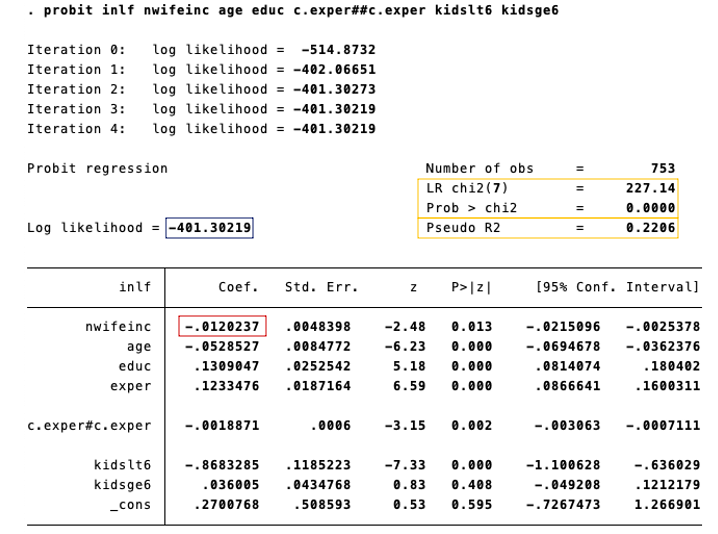
\includegraphics[scale=0.4]{images/ProbitStata.png}
    \label{fig:my_label}
\end{figure}    
\end{frame}

\begin{frame}{Logit}
    \begin{figure}[H]
    \centering
    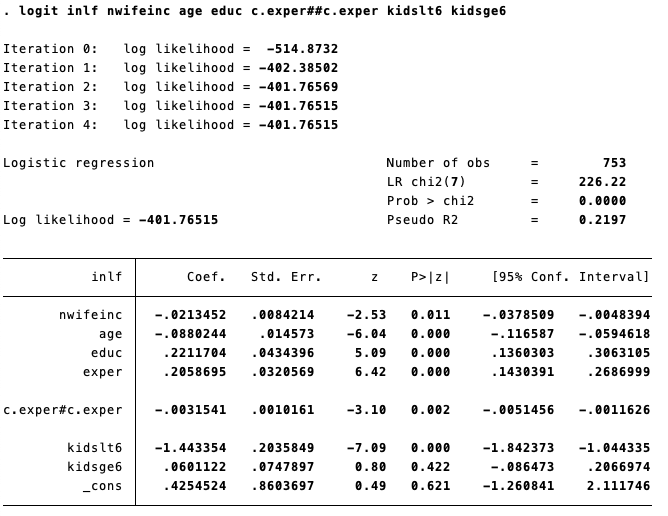
\includegraphics[scale=0.4]{images/LogitStata.png}
    \label{fig:my_label}
\end{figure}
\end{frame}

% \begin{frame}{Pseudo-R2 in Maximum Likelihood Regression}
%   \begin{itemize}
%     \item Unlike traditional R-squared in ordinary least squares (OLS) regression, MLE does not have a direct equivalent. Therefore, pseudo-R2 measures are employed.
%         \item Pseudo-R2 and Likelihood Function:
%       \begin{itemize}
%         \item Adding regressors increases maximized likelihood, similar to OLS.
%         \item Compares maximized likelihood with all regressors to that with none (Bernouilli).
%       \end{itemize}
%         \item Easy to understand BUT Doesn't reflect prediction quality; treats 51\% and 90\% predictions equally.
% \item Commonly used pseudo-R2 measures in MLE include:
%       \begin{itemize}
%         \item McFadden (1974)'s $R^2$: $\Bigg[1 - \frac{\text{Log-Likelihood of Model}}{\text{Log-Likelihood of Null Model}}\Bigg]$
%         \item Cox and Snell (1989) $R^2$:$ \Bigg[1 - \left( \frac{\text{Log-Likelihood of Model}}{\text{Log-Likelihood of Null Model}} \right)^{\frac{2}{n}}\Bigg]$
%         \item Nagelkerke (1991)'s $R^2$: An adjustment to Cox and Snell for improved scaling.
%       \end{itemize}
%   \end{itemize}
% \end{frame}

\begin{frame}{Summary and Conclusion}
  \begin{itemize}
    \item If $Y_i$ is binary, $\mathbb{E}(Y\mid X)=Pr(Y=1\mid X)$
    \item Three models: 
    \begin{itemize}
        \item linear probability model (linear multiple regression)
        \item probit (cumulative standard normal distribution)
        \item logit (cumulative standard logistic distribution)
    \end{itemize}
    \item LPM, probit, logit all produce predicted probabilities
    \item Effect of $\Delta X$ is the change in conditional probability that $Y=1$. But for logit and probit, this depends on the initial $X$
    \item Probit and logit are estimated via maximum likelihood
  \begin{itemize}
    \item Coefficients are normally distributed for large n
    \item Large-n hypothesis testing, conf. intervals is as usual
  \end{itemize}
  There are many models for limited dependent variables, other than binary variables,  in econometric applications.
  \begin{itemize}
    \item Discrete choice or multiple choice data (multinomial probit/logit)
    \item Censored Data Models (Tobin's Tobit)
    \item Truncated Data Models (Heckman's Sample Selection)
    \item Count Data Models (Poisson and Negative Binomial)
    \item Ordered response data (Ordered probit/logit)
  \end{itemize}

  \end{itemize}
\end{frame}



\begin{frame}[allowframebreaks]{Material}
\begin{itemize}
    \item[--] \textbf{Textbooks:}
    \begin{itemize}
        \item Introduction to Econometrics, 4th Edition, Global Edition, by Stock and Watson -- Chapters 11
    \end{itemize}
\end{itemize}
\end{frame}

\end{document}
